\subsection{Mô hình hoạt động, tương tác và miền dữ liệu}
Ba hình dưới mô tả luồng đặt/thanh toán và mô hình miền ở mức chọn lọc, không thay thế kiểm thử hoặc chứng minh triển khai. Nguồn PlantUML và ảnh render được lưu cùng nhau tại \texttt{docs/diagrams/}. Voucher biểu diễn chính sách mã giảm giá; sổ LoyaltyTransaction lưu biến động điểm. Class diagram rút gọn thuộc tính, không phải bản sao đầy đủ schema.
\begin{figure}[p]\centering
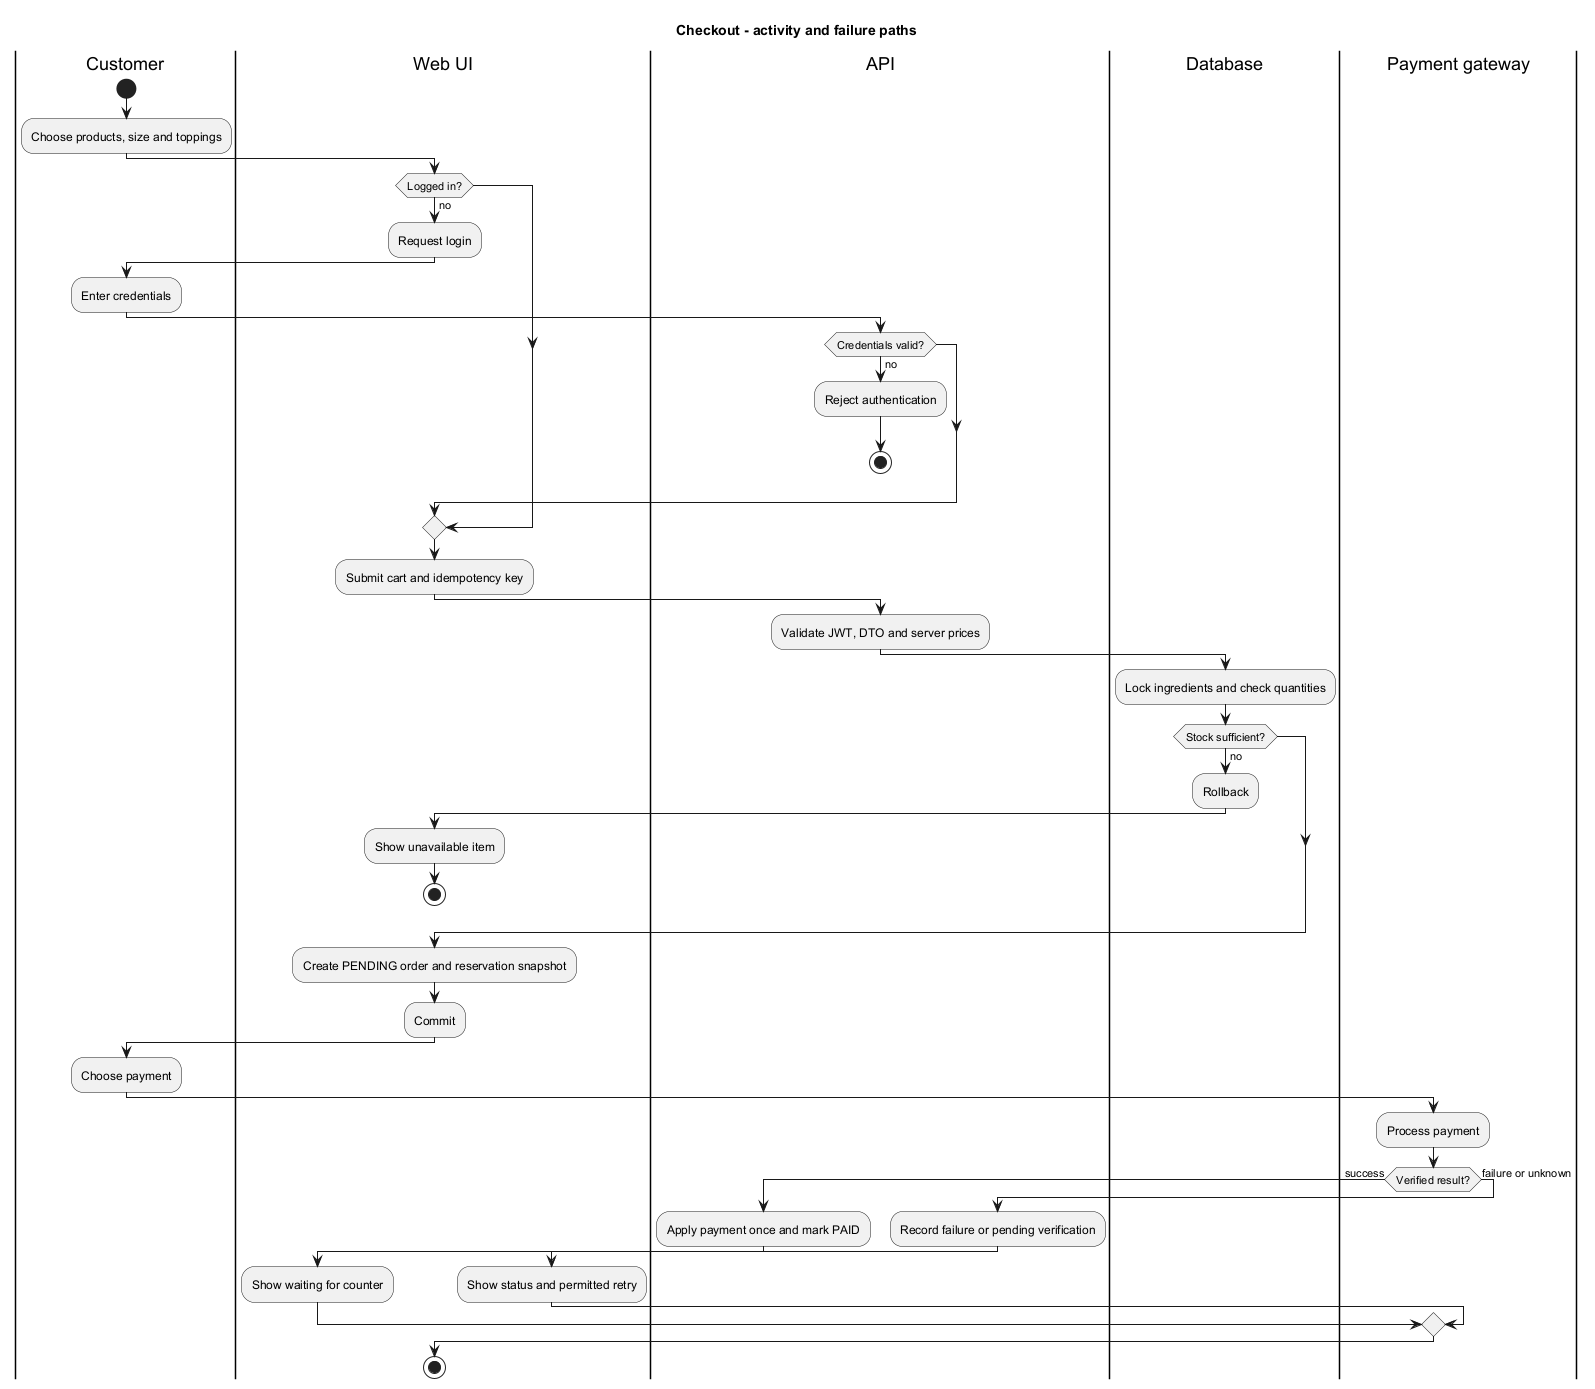
\includegraphics[width=\linewidth,height=.82\textheight,keepaspectratio]{../docs/diagrams/activity-checkout.png}
\caption{ACT-01: hoạt động đặt hàng với swimlane và nhánh chưa đăng nhập, hết kho, thanh toán lỗi}
\end{figure}
\begin{figure}[p]\centering
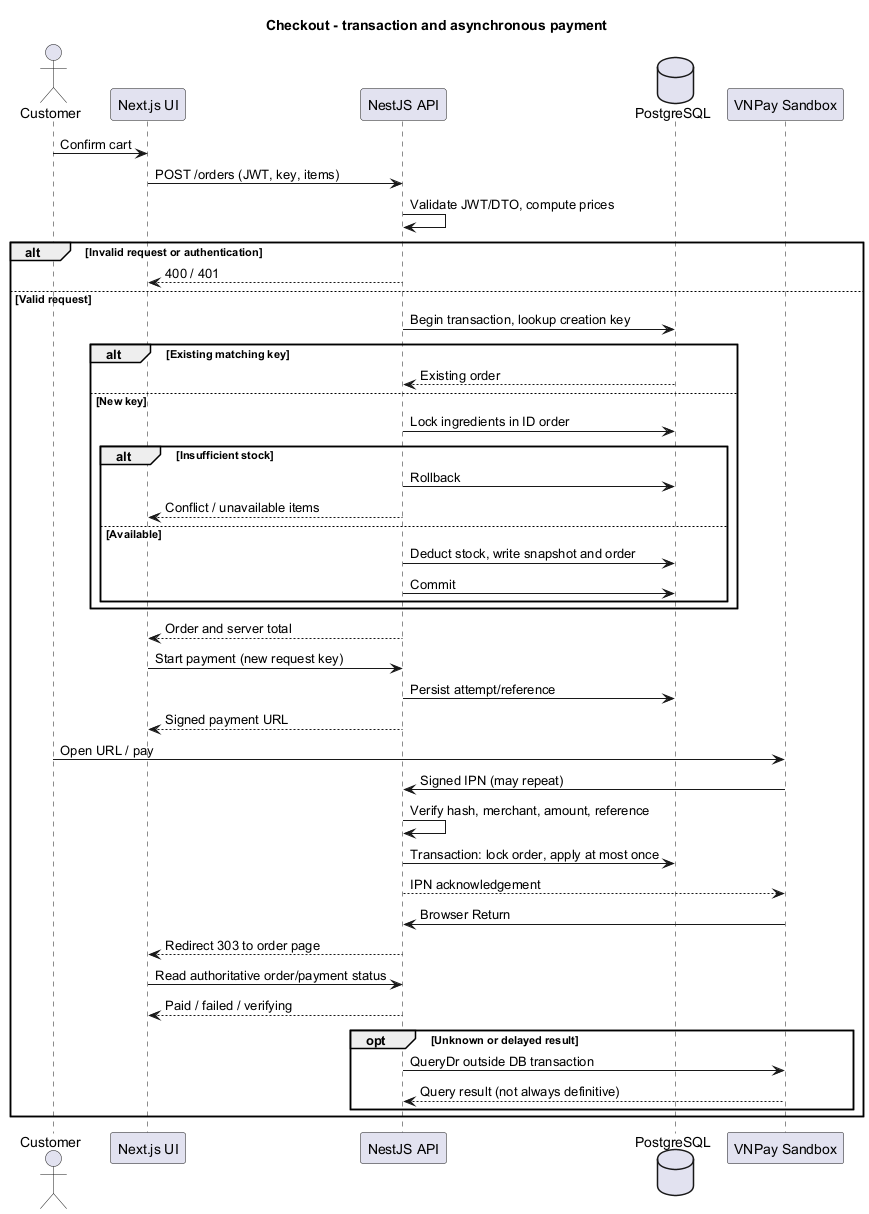
\includegraphics[width=\linewidth,height=.82\textheight,keepaspectratio]{../docs/diagrams/sequence-checkout.png}
\caption{SEQ-01: tương tác UI, API, database và gateway; transaction và callback bất đồng bộ}
\end{figure}
\begin{figure}[p]\centering
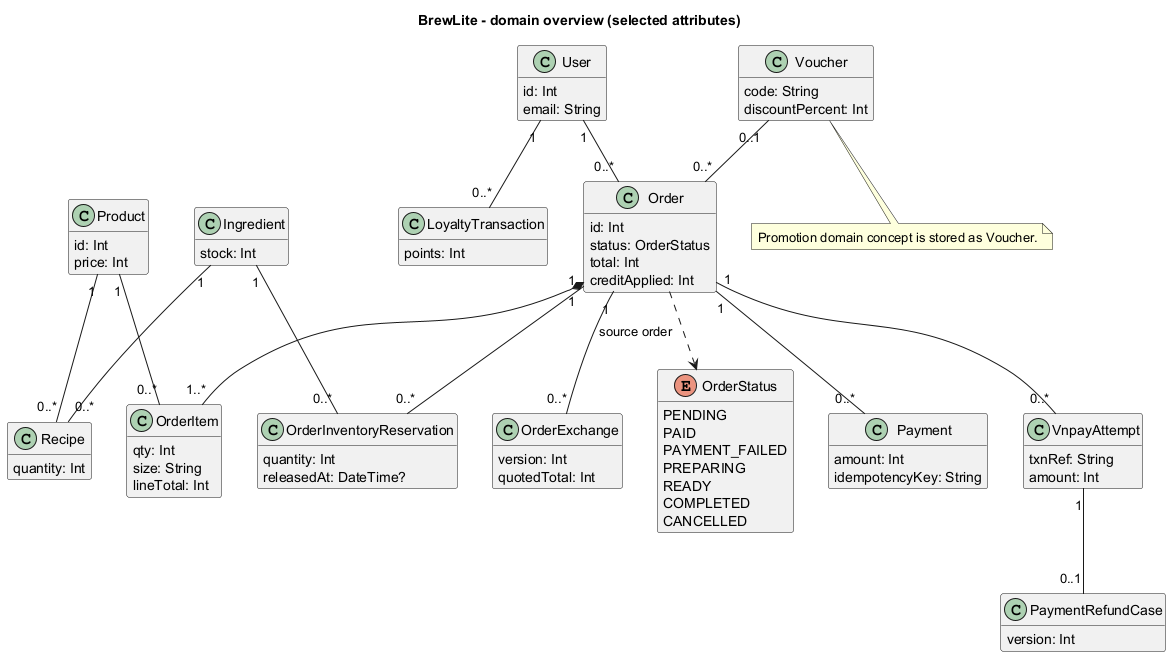
\includegraphics[width=\linewidth,height=.82\textheight,keepaspectratio]{../docs/diagrams/class-domain.png}
\caption{CLASS-01: các thực thể chính, quan hệ và bội số}
\end{figure}
\clearpage
